\documentclass[a4j,11pt]{jarticle}

\usepackage[top=25truemm,  bottom=30truemm,
            left=25truemm, right=25truemm]{geometry}


\title{工学基礎実験実習 \\
       レポート文書作成技術 第 2 回レポート\\─ ニュートン法に関する実験 ─}

\author{氏名: 重近 大智 (SHIGECHIKA, Daichi) \\
        学生番号: 09501527}

\date{出題日: 2019年6月4日 \\
      提出日: 2019年6月4日 \\
      締切日: 2019年6月11日 \\}

\usepackage{graphicx}
\begin{document}
\maketitle
\tableofcontents
\section{はじめに}
方程式の求解は,科学技術計算において頻繁に現れる.解の公式が存在する方程式では,有限回の四則演算と初等関数によって解を計算できるが,一般の方程式の解を解析的に表す公式は存在しない.このような場合は,解の近似値を計算する数値解法が有用である.ニュートン法\cite{author1,author3}は代表的な数値解法である.多くの場合,ニュートン法は2次の収束を示すため,効率良く解を得ることができる.ただし,ニュートン法は初期値として解の粗い近似値を与える必要があり,初期値が適切でない場合,収束までに多くの反復を要したり,収束しない場合もある.また,計算しようとしている解が重解である場合は,収束が遅くなる.ニュートン法の使用に際しては,このような欠点に留意する必要がある.
以下では,ニュートン法の挙動を理論的に解析し,$f(x)=(x-1)(x+1)^2=0$を対象として,ニュートン法の性質を調べる実験を行う.
\section{ニュートン法の原理}
方程式$f(x)=0$の{\em 解}とは,関数$f(x^*)=0$を満たす$x^*$のことを言う.図\ref{fig:newton}では,曲線$y=f(x)$と$x$軸が交わっており,この交点の座標が$x^*$である.

いま,解$x^*$の近似値$x_k$が与えられているとする.点$(x_k,f(x_k))$における曲線$y=f(x)$の接線(図中の斜めの線)の方程式は$y=f(x_k)+(x-x_k)\cdot f^\prime(x_k)$である.ここで,$f^\prime(x)$は$f(x)$の導関数である.この接線と$x$軸の交点$(x_{k+1})$は次の式で表される\cite{author2,author3}.
\begin{equation}
x_{k+1}=x_k-\frac{f(x_k)}{f'(x_k)}
\label{eq:newton}
\end{equation}
\begin{figure}
\begin{minipage}[b]{210pt}
\center
\begin{verbatim}
$ python3.6
>>> x=1.1
>>> x=x-(x-1)*(x+1)*(x+1)/(3*x*x+2*x-1);x
1.008695652173913
>>> x=x-(x-1)*(x+1)*(x+1)/(3*x*x+2*x-1);x
1.0000746407911925
>>> x=x-(x-1)*(x+1)*(x+1)/(3*x*x+2*x-1);x
1.000000005570624
>>> x=x-(x-1)*(x+1)*(x+1)/(3*x*x+2*x-1);x
1.0
>>> x=x-(x-1)*(x+1)*(x+1)/(3*x*x+2*x-1);x
1.0
\end{verbatim}
\caption{実験結果1}
\label{result}
\end{minipage}
\begin{minipage}[b]{250pt}
\center
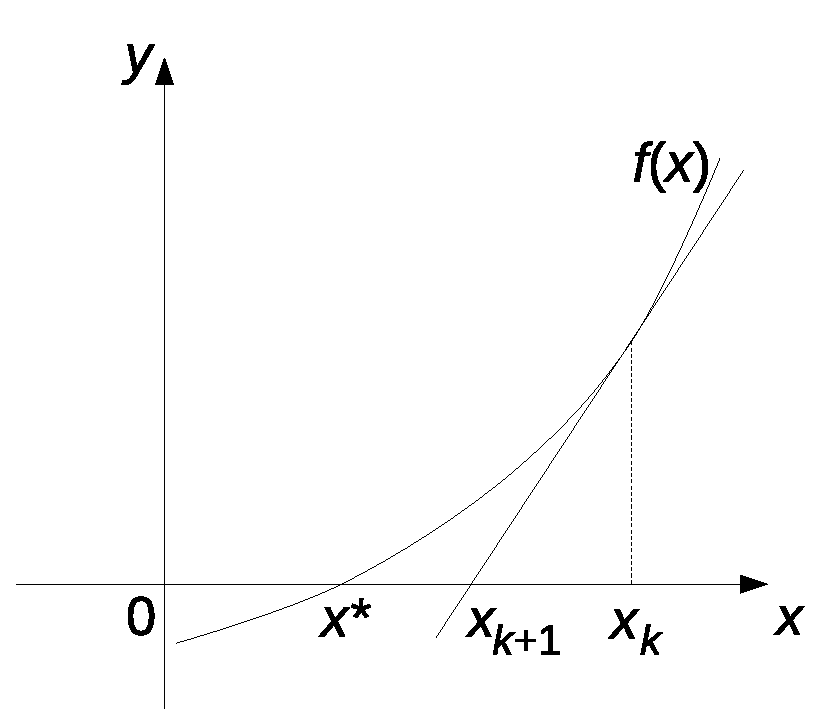
\includegraphics[scale=0.5]{figure3.eps}
\caption{ニュートン法の幾何学的解釈}
\label{fig:newton}
\end{minipage}
\end{figure}
図\ref{fig:newton}の場合,$x_{k+1}$が$x_k$よりも解$x^*$に近い.このため,適当な初期値$x_0$を与え,式\ref{eq:newton}によって数列($x_k$)を定義すると,この数列は$k\rightarrow \infty$で$x^*$に{\em 収束}することが期待される.

収束性の議論を厳密にするために,極限値$x^*$との誤差$r_k$を次のように定義する.
\begin{equation}
r_k:=x_k-x^*
\label{eq:syuusoku}
\end{equation}
式\ref{eq:newton}の関数$f(x)$を$x^*$の近傍でテイラー展開して,整理すると次式が得られる\cite{author1}.
\begin{equation}
r_{k+1}=r_k-\left. \frac{r_kf^\prime+r^2_kf^{\prime\prime}/2+\cdots}{f^\prime+r_kf^{\prime\prime}+\cdots} \right|_{x=x^*}
=(r^2_k/2)(f^{\prime\prime}/f^\prime)\|_{x=x^*}+O(r^3_k)
\label{eq:taylor}
\end{equation}
ただし,$f^\prime(x_k)\neq 0$と仮定した.上の式は$r_{k+1}$が$r^2_k$に比例することを示している.これを2次収束という.これは,$r_k$が十分に小さければ,式(\ref{eq:newton})の適用によって,正しい桁数がほぼ2倍になることを示している.逆に,$r_k$が大きいときや$f^\prime(x_k)$が$0$に近いときには発散する場合がある.また,$f^\prime(x_k)=0$のときは$x_{k+1}$が計算できない.

なお,重解の場合($f^\prime(x^*)=0$の場合)は1次収束である.また,解付近で2次導関数が$0$になる場合には3次の収束を示す.

\section{実験}
ここでは,次の方程式(図\ref{1})にニュートン法を適用して,挙動を調べる.
\begin{equation}
f(x)=(x-1)(x+1)^2
\label{eq:fx}
\end{equation}
\begin{figure}
\begin{minipage}[t]{200pt}
\center
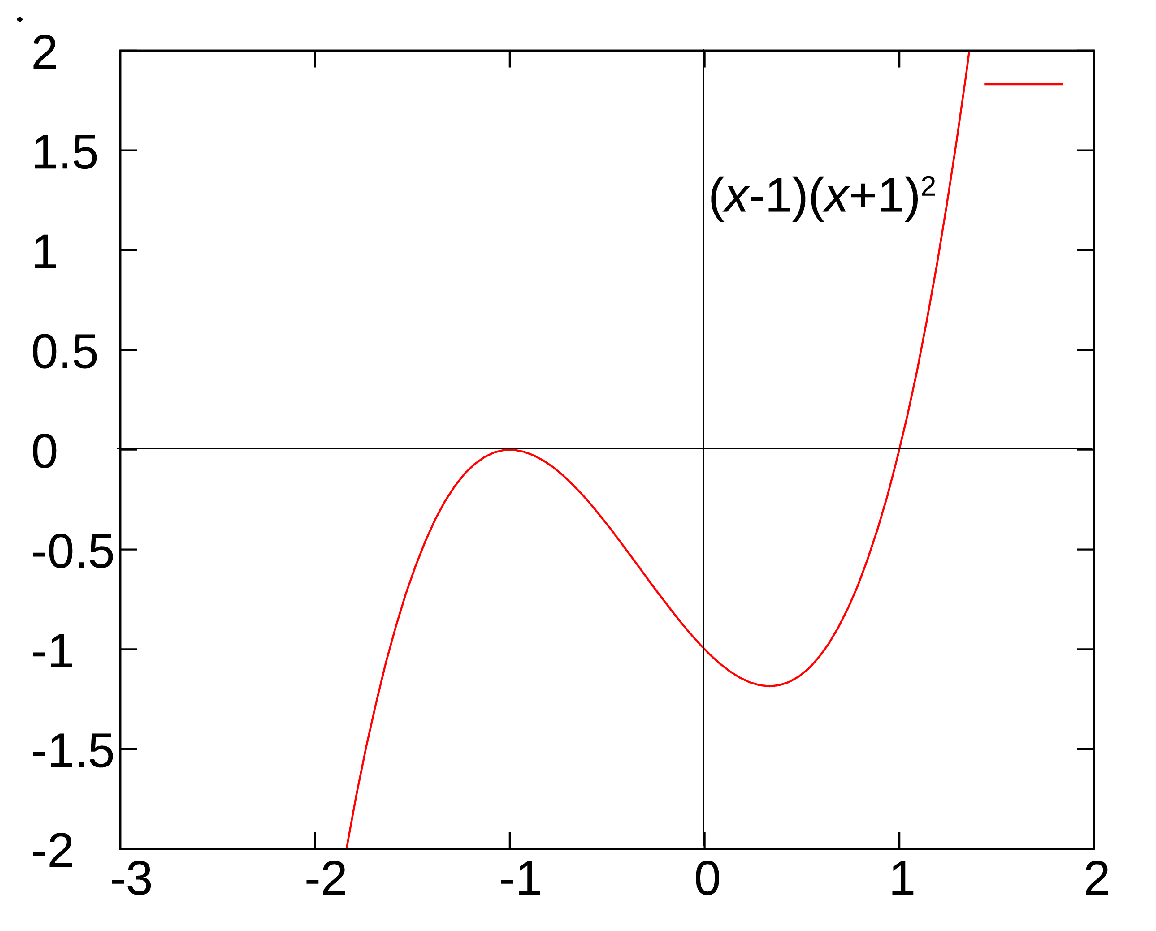
\includegraphics[scale=0.35]{newton3.eps}
\caption{$(x-1)(x+1)^2のグラフ$}
\label{1}
\end{minipage}
\begin{minipage}[t]{230pt}
\center
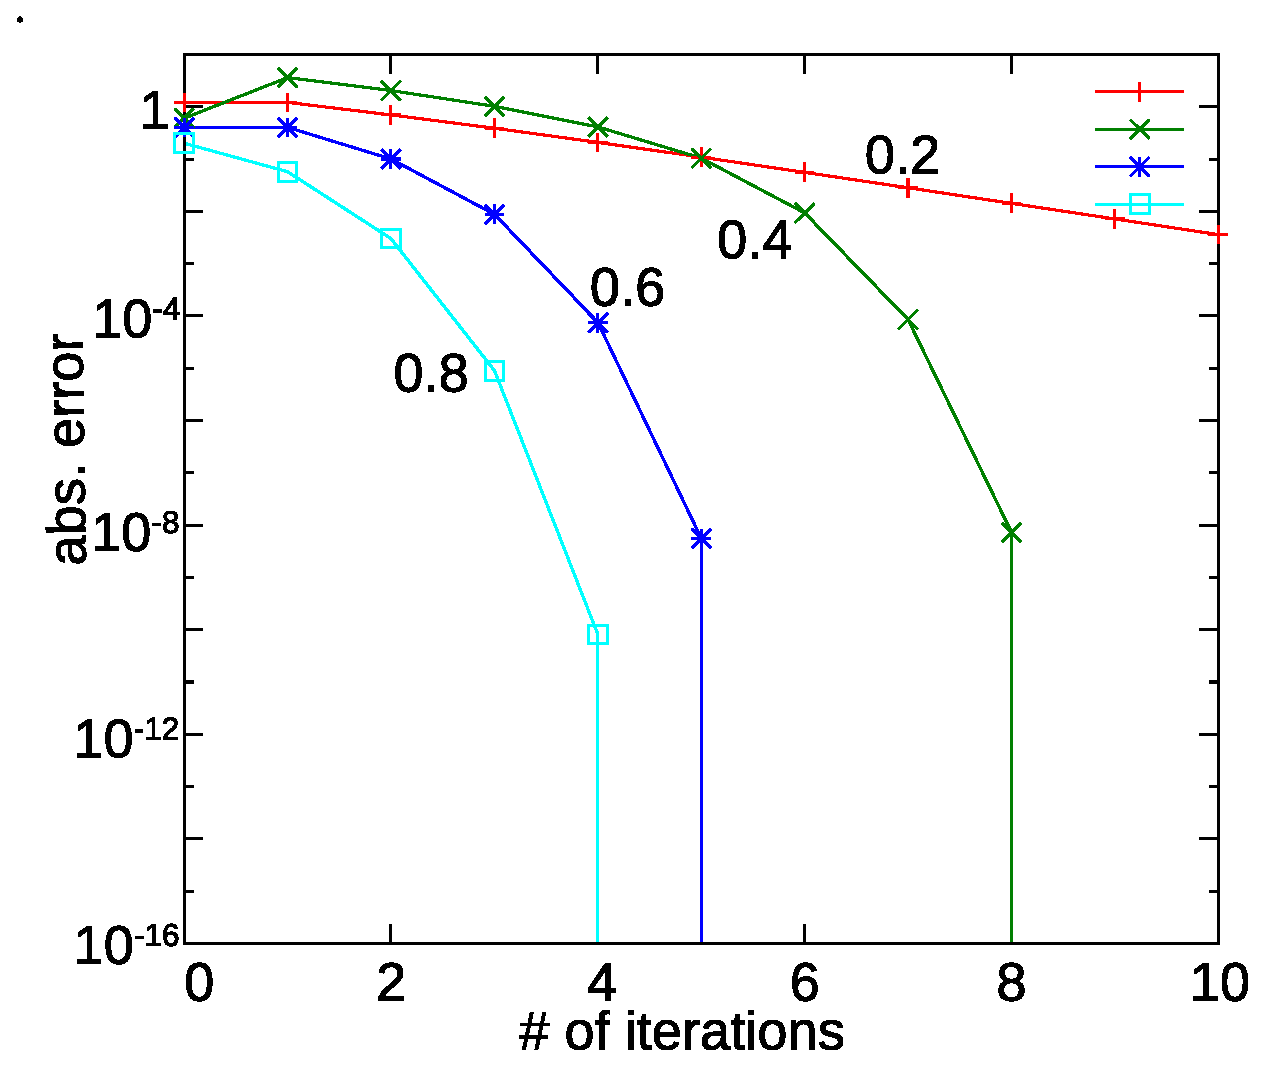
\includegraphics[scale=0.35]{newtonresult2.eps}
\caption{反復回数と誤差の関係}
\label{newtonresult}
\end{minipage}
\end{figure}
解は,$1$,$-1$,$1$である.導関数は$3x^2+2x-1$であるからニュートン法の反復式は次のようになる.
\begin{equation}
x_{k+1}=x_k-(x_k-1)(x_k+1)^2/(3x^2_k+2x_k-1)
\label{newtonrepeat}
\end{equation}
初期値を1.1とし,bcコマンドを用いてニュートン法の反復を行った結果を図\ref{result}に示す.5回の反復で約20桁まで正しく得られていることがわかる.初期値が10の場合には11回の反復を要した.

初期値を$-2$とすると重解の$-1$に近づく.しかし,10反復後の$x_{10}$が$-1.0014\cdots$であり,2桁程度しか正しくない.20桁程度の精度に達するには数十回の反復を要すると考えられる.しかし,実際には30数回目以降は桁落ちのため正しく計算されなかった.

表\ref{table}に,様々な初期値からニュートン法の反復を10回行った後の値を示す.$f^\prime(x)=0$となるのは$x=-1,1/3$であるため,$x_k$が$-1$または$1/3$となってはならない.概ね,初期値が$1/3$を越える場合は$1$に収束すると考えられる.また,この場合は2次収束なので,10回以内の反復で収束している.一方,初期値が$1/3$より小さい場合には,重解$-1$に向かうが,1次収束であるため10回の反復では2桁程度の精度しか得られない.初期値が$0$の場合は次に$x_1=-1$となり,それ以上計算できないためN/A(not available)と表示している.

図4に,様々な初期値に対する誤差$r_k$の絶対値の推移を対数目盛を示す.各折れ線付近の数字は初期値を表す.bcの性質上,最後の値は$10^{-20}$の誤差を含んでいるため,折れ線の一番右側が正しくない形に曲がっているが,初期値が$0.4$以上の場合(解1に2次収束する場合)は,ほぼ同じ形状で急速に誤差が減少していることが分かる.一方,初期値が$0.2$の場合(解$-1$に1次収束する場合)は,直線を描いており,この直線が$10^{-20}$に達するには非常に時間が掛かることが用意に予想できる.
\begin{table}[t]
\center
\caption{様々な初期値からのニュートン法の反復結果}
\begin{tabular}{|c|c|}
\hline
初期値&10回の反復後の値\\
\hline
-0.2&−0.99964988198316793008\\
0&N/A\\
0.2&−1.00357177068625731955\\
0.4&1.00000000000000000001\\
0.6&1.00000000000000000001\\
0,8&1.00000000000000000001\\
\hline
\end{tabular}
\label{table}
\end{table}
上記の初期値では誤差は単調に減少しているが,一般には誤差が増加することもあり得る.$x_k$が$1/3$付近または$-1$付近の値をとる場合には,$f^\prime(x_k)$が0に近いため$x_{k+1}$が非常に大きな値となり,誤差が増大する.このため,ニュートン法の初期値$x_k$がこのような際どい領域を通過しないように選ぶ必要がある.
\section{まとめ}
ここでは,簡単な方程式にニュートン法を適用し,解と極限値の関係を調べた.また,挙動の理論的解析を行った.

実際の応用では,解のわからない難しい方程式を解く必要がある.このような問題については,今後の更なる検討を要する.
\section{修正点}
\begin{itemize}
\item 目次を追加した.
\item 段落の初めの空き文字数が2文字になっていたのを1文字に修正した. 
\item tableやfigureで[h]を使用していたのをなくした.
\item 表のキャプションを表の上側に移動した.
\item 図中の文字の大きさを変更した.
\item minipageを用いて図表を横に並べた.
\item ・をcdotに変更した.
\item $'$をprimeに変更した.
\item 改行をbigskipに変更した.
\item 誤字を修正した.
\end{itemize}
\begin{thebibliography}{99}
\bibitem{author1} 著者1,著者2,数値計算の基礎,某出版社,2005.
\bibitem{author2} Cox D.A., Little J. and O'Shea D.,Using Algebraic Geometry, Springer, 2005.
\bibitem{author3} http://mathworld.wolfram.com/NewtonsMethod.html
\end{thebibliography}
\end{document}
